\chapter{Organisation du travail}

\section{Répartition des tâches}

Comme le projet peut être découpé en plusieurs blocs qui peuvent être
développés de manière presque indépendante, nous nous sommes répartis
par équipe sur chaque bloc. Certains blocs nécessitent
cependant une base provenant d’autres blocs pour faire des tests.
Par exemple, la partie IHM aura besoin d’une base de données pour
vérifier que la recherche d’imagettes dans celle-ci se déroule bien.
Nous allons donc commencer par développer des prototypes simplifiés
pour que tout le monde puisse améliorer sa partie.

\paragraph{}
Voici la répartition que nous avons effectuée sur les différents blocs :

\begin{center}

\begin{tabular}{ | l | l | }
	\hline
	\multicolumn{2}{ | c | }{ \textbf{Bloc 1 : Préparation des données} } \\
	\hline
	\textbf{Spécification} & \textbf{Description} \\
	\hline
	PR\_FO\_1 & Traiter le format PiFF en interne dans le logiciel \\
	\hline
	PR\_FO\_2 & Fournir un convertisseur du format GEDI vers PiFF \\
	\hline
	PR\_TR\_1 & Intégrer une fonction de détection de lignes au logiciel \\
	\hline
	PR\_TR\_2 & Permettre un découpage des images en lignes \\
	\hline
	PR\_TR\_3 & Localiser les paragraphes \\
	\hline
	PR\_TR\_4 & Permettre un découpage des images en paragraphes \\
	\hline
	PR\_RE\_1 & Associer les images à leur transcription \\
	\hline
	PR\_RE\_2 & Associer la vérité terrain à une transcription \\
	\hline
	PR\_RE\_3 & Permettre de générer une vérité terrain si besoin, grâce à un reconnaisseur \\
	\hline
\end{tabular}

\paragraph{}
\begin{tabular}{ | l | l | }
	\hline
	\multicolumn{2}{ | c | }{ \textbf{Bloc 2 : Stockage des données} } \\
	\hline
	\textbf{Spécification} & \textbf{Description} \\
	\hline
	STO\_VER & Stocker des imagettes associées à une vérité terrain \\
	\hline
	STO\_USR & Stocker des imagettes associées à une transcription générée par l’utilisateur \\
	\hline
	STO\_REC & Stocker des imagettes associées à une transcription générée par un reconnaisseur  \\
	\hline
	STO\_SEL & Fournir des méthodes pour accéder aux données stockées  \\
	\hline
	STO\_UPD & Fournir des méthodes pour modifier les données stockées \\
	\hline
	STO\_INS & Fournir des méthodes pour pouvoir insérer des données à stocker \\
	\hline
	STO\_DEL & Fournir des méthodes pour pouvoir supprimer des données stockées \\
	\hline
\end{tabular}

\paragraph{}
\begin{tabular}{ | l | l | }
	\hline
	\multicolumn{2}{ | c | }{ \textbf{Bloc 3 : Interface avec le reconnaisseur} } \\
	\hline
	\textbf{Spécification} & \textbf{Description} \\
	\hline
	IR\_CV & Convertir les données au format d’entrée du reconnaisseur \\
	\hline
	IR\_AP & Fournir les données au reconnaisseur \\
	\hline
	IR\_EV & Pouvoir lancer une évaluation du reconnaisseur  \\
	\hline
	IR\_TR & Pouvoir lancer une transcription d’un document par le reconnaisseur   \\
	\hline
\end{tabular}

\paragraph{}
\begin{tabular}{ | l | p{0.8\linewidth} | }
	\hline
	\multicolumn{2}{ | c | }{ \textbf{Bloc 4 : Interface avec l’utilisateur} } \\
	\hline
	\textbf{Spécification} & \textbf{Description} \\
	\hline
	PEA\_GEN\_1 & Naviguer entre les différents documents d’un même classeur \\
	\hline
	PEA\_GEN\_2 & Naviguer entre les différentes pages du manuscrit en cours d’annotation \\
	\hline
	PEA\_GEN\_3 & Basculer vers la page d’édition des zones de découpe à l’aide d’un bouton \\
	\hline
	PEA\_GEN\_4 & Posséder une zone montrant la page découpée afin de localiser les zones de découpe du manuscrit, avec la zone en cours d’annotation figurant en une couleur différente \\
	\hline
	PEA\_GEN\_5 & Afficher la liste des imagettes du manuscrit découpé \\
	\hline
	PEA\_GEN\_6 & Modifier directement la base de données quand on modifie une vérité terrain \\
	\hline
	PEA\_GEN\_7 & Supprimer un couple imagette-transcription de la base de données à l’aide d’un bouton prévu à cet effet \\
	\hline
	PEA\_GEN\_8 & Ajouter à la base de données des documents avec ou sans transcription \\
	\hline
	PEA\_GEN\_9 & Exporter les données validées afin de lancer un nouvel apprentissage \\
	\hline
	PEA\_MA\_1 & Placer le curseur sur la première imagette ne possédant pas de transcription à l’ouverture de la page \\
	\hline
	PEA\_MA\_2 & Un appui sur la touche Entrée permet de positionner le curseur sur l’annotation suivante \\
	\hline
	PEA\_MA\_3 & Proposer un bouton permettant de basculer vers la prochaine imagette sans vérité-terrain \\
	\hline
	PEA\_MCR\_1 & Un appui sur Entrée valide les transcriptions zone par zone et passe à la zone suivante \\
	\hline
	PEA\_MCR\_2 & Modifier une transcription en cliquant dessus pour y positionner le curseur et effectuer manuellement les modifications  \\
	\hline
	PEA\_MV\_1 & Un appui sur Entrée valide les transcriptions zone par zone \\
	\hline
	PEA\_MV\_2 & Modifier une transcription en cliquant dessus pour y positionner le curseur et effectuer manuellement les modifications  \\
	\hline
	PDEC\_OD\_1 & Créer une nouvelle zone à l’aide d’un rectangle \\
	\hline
	PDEC\_OD\_2 & Les zones ne sont donc pas limitées à des rectangles, mais peuvent prendre la forme d’autres polygones \\
	\hline
	PDEC\_OD\_3 & Déplacer la zone sélectionnée sur le manuscrit \\
	\hline
	PDEC\_OD\_4 & Zoomer et dézoomer sur le manuscrit  \\
	\hline
	PDEC\_OD\_5 & Annuler la dernière action \\
	\hline
	PDEC\_OD\_6 & Refaire l’action annulée précédemment \\
	\hline
	PDEC\_OD\_7 & Supprimer toutes les zones de la page pour retourner au manuscrit vierge \\
	\hline
	PDEC\_OD\_8 & Proposer une option “appliquer la détection de lignes sur la zone” \\
	\hline
	PDEC\_OD\_9 & Valider la découpe et basculer vers la page d’édition des annotations  \\
	\hline
	PDEC\_VM\_1 & Posséder un bouton de retour au menu principal \\
	\hline
	PDEC\_VM\_2 & Permettre à l’utilisateur d’ouvrir un autre manuscrit \\
	\hline
	PDEC\_VM\_3 & Permettre de naviguer entre les différentes pages du manuscrit \\
	\hline
	PDEC\_VM\_4 & Permettre à l’utilisateur de se déplacer sur le manuscrit horizontalement et verticalement à l’aide d’un bouton de défilement \\
	\hline
\end{tabular}

\paragraph{}
\begin{tabular}{ | l | l | }
	\hline
	\multicolumn{2}{ | c | }{ \textbf{Bloc 5 : Général} } \\
	\hline
	\textbf{Spécification} & \textbf{Description} \\
	\hline
	GEN\_ERGO & Ergonomie de l‘application \\
	\hline
	GEN\_ERGO & Concevoir un logiciel évolutif \\
	\hline
	GEN\_ERGO & Fournir un logiciel open source \\
	\hline
\end{tabular}

\end{center}

\paragraph{}

Ainsi nous nous répartissons le travail selon ces blocs.
Enzo Crance et Valentin Fouche s’occupent du bloc 1, Kevin Despoulains et Corentin Guilloux du bloc 2, Timothée Neitthoffer du bloc 3, Laure Du Mesnildot et Charlotte Richard du bloc 4 et Gaël Gendron du bloc 5. 

\paragraph{}
Cette répartition des tâches permet à chaque équipe de spécifier plus en détail
sa partie, et donc de pouvoir estimer plus précisément le temps que prendra le
développement. Nous espérons donc avoir un rapport de planification précis qui
nous permettra d’anticiper d’éventuelles réorganisations d’équipes en fonction
des différentes charges de travail.

\section{Organisation temporelle}

Certains membre du groupe partent en mobilité en Janvier (Kévin DESPOULAINS,
Corentin GUILLOUX, et Gaël GENDRON). Notre premier objectif est donc de
concevoir la base et la documentation de chaque partie avant leur départ.
Nous allons donc anticiper la phase de développement en la débutant dès à
présent. Le diagramme de Gantt précédemment établi se trouve donc modifié de
cette manière :

\paragraph{}
\begin{mdframed}[frametitle={Figure 12 : Estimation de la planification des tâches}, innerbottommargin=10]
\begin{center}
%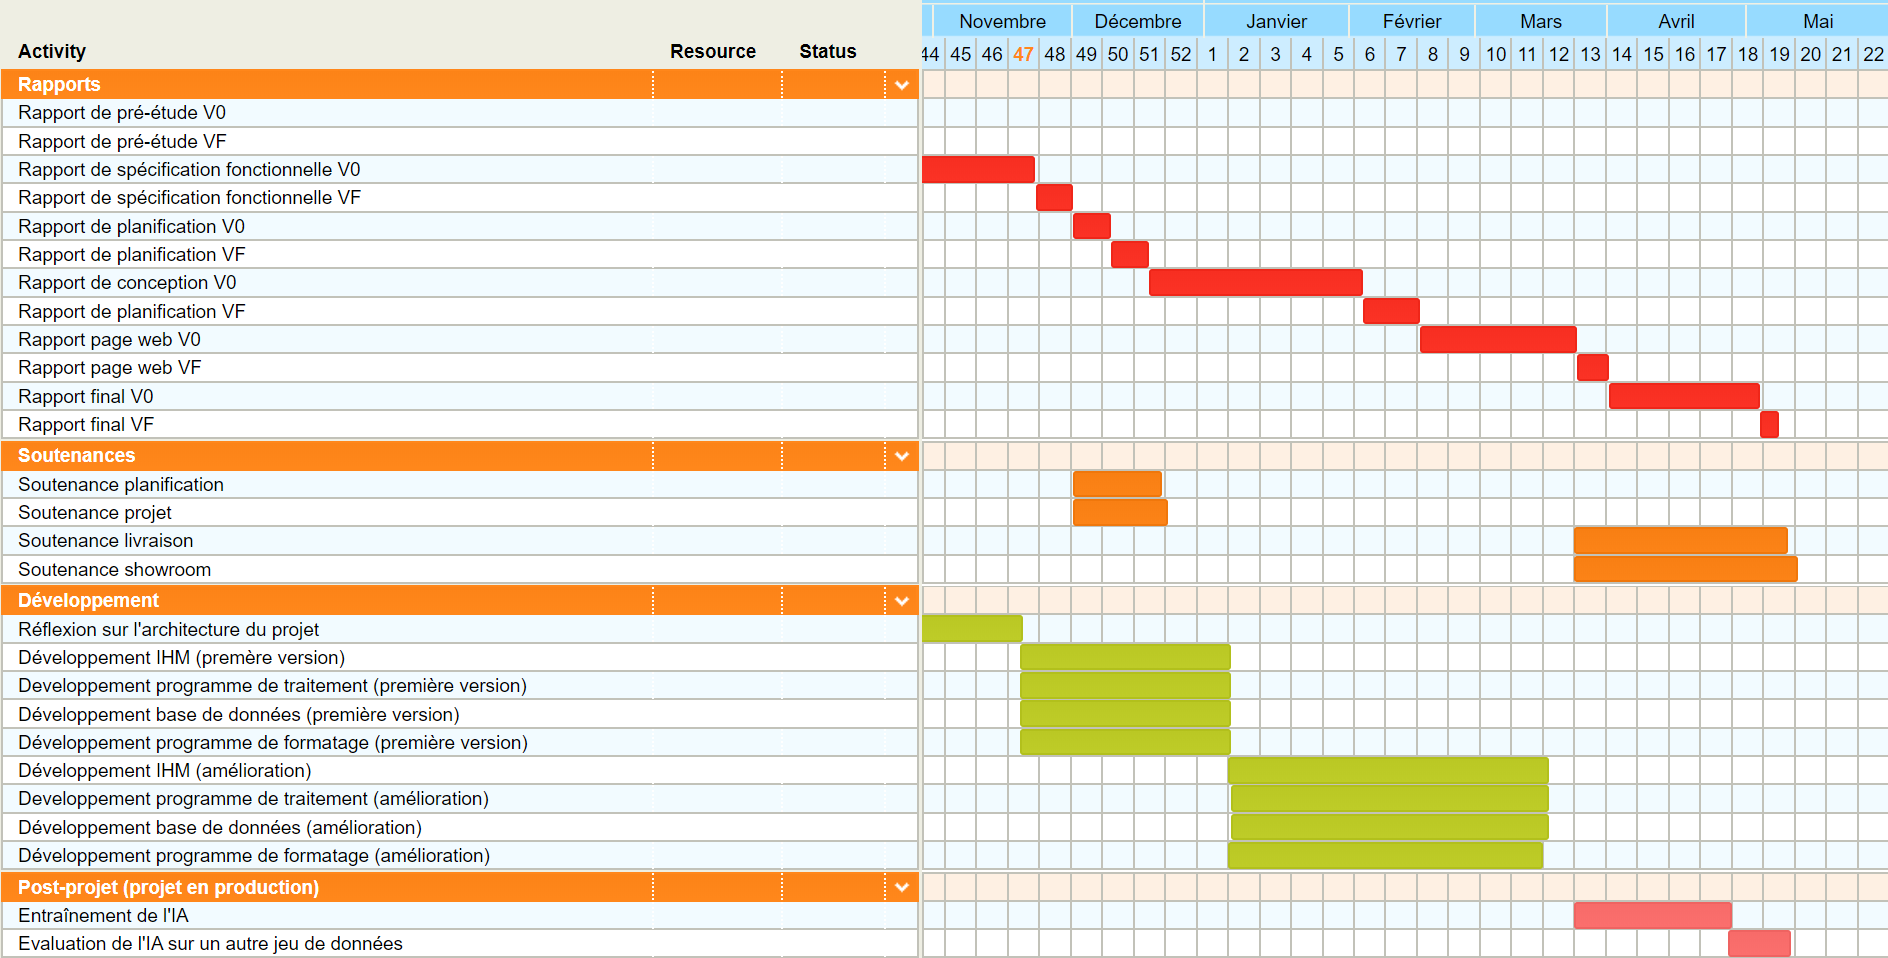
\includegraphics[scale=0.6]{gantt.png}
\end{center}
\end{mdframed}

\paragraph{}
\underline{Légende}

\paragraph{}
\textcolor{red}{En rouge : } rédaction des différents livrables. Nous avons estimé que le début de rédaction d’un livrable doit se faire dès le rendu du livrable précédent.

\paragraph{}
\textcolor{orange}{En orange : } soutenances. Les dates de début de préparation sont pour l’instant difficiles à définir, la taille des blocs est donc provisoire.

\paragraph{}
\textcolor{green}{En vert : } développement. Comme on peut le voir, il y a plusieures parties du développement qui se font en parallèle. Les durées de chaques parties sont prévisionnelles mais sont susceptibles d’être grandement modifiées.

\paragraph{}
\textcolor{pink}{En rose : } exécution du projet en mode production. Ce seront les tests du reconnaisseur.